\documentclass{article} % 1. 必须定义文档类

% 2. 必须加载必要的宏包
\usepackage{tikz}
\usetikzlibrary{arrows.meta, positioning}
\usepackage[utf8]{inputenc} % 支持编码
\usepackage{xeCJK}          % 如果你用 XeLaTeX 编译中文，必须加上这个

\begin{document} % 3. 必须进入 document 环境

\begin{figure}[t]
\centering
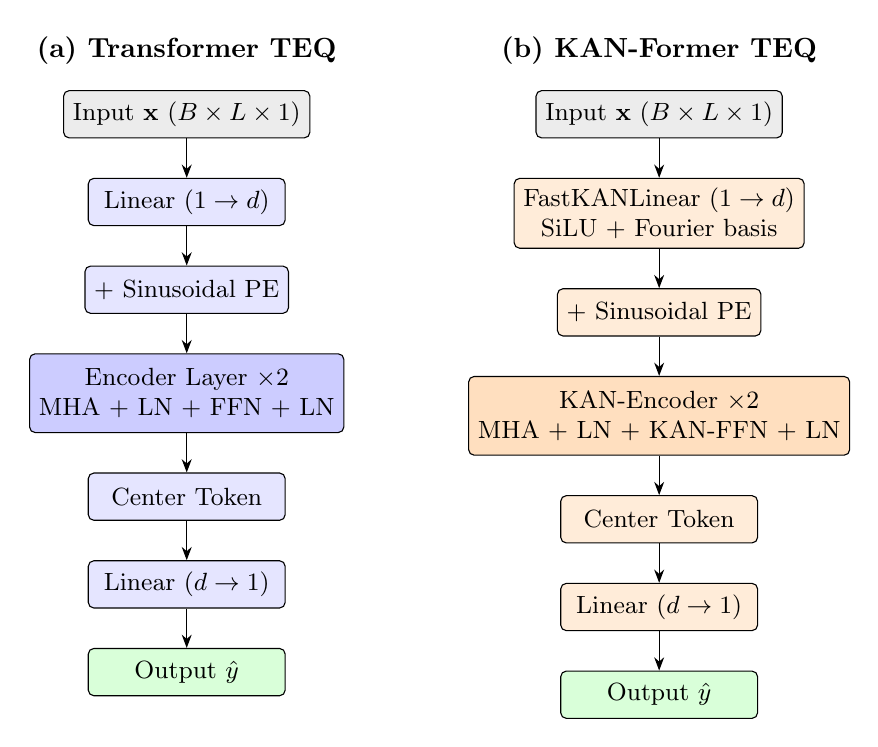
\begin{tikzpicture}[
  node distance=0.5cm,
  block/.style={rectangle, draw, rounded corners=2pt, minimum width=2.5cm, minimum height=0.6cm, align=center, font=\small},
  arrow/.style={-Stealth}
  ]
  % ========== 左图: Transformer TEQ ==========
  \begin{scope}[local bounding box=left]
    \node[block, fill=gray!15] (L0) {Input $\mathbf{x}$ ($B \times L \times 1$)};
    \node[block, below=of L0, fill=blue!10] (L1) {Linear ($1 \to d$)};
    \node[block, below=of L1, fill=blue!10] (L2) {+ Sinusoidal PE};
    \node[block, below=of L2, fill=blue!20, minimum height=1cm] (L3) {Encoder Layer $\times 2$ \\ MHA + LN + FFN + LN};
    \node[block, below=of L3, fill=blue!10] (L4) {Center Token};
    \node[block, below=of L4, fill=blue!10] (L5) {Linear ($d \to 1$)};
    \node[block, below=of L5, fill=green!15] (L6) {Output $\hat{y}$};
    \draw[arrow] (L0) -- (L1); \draw[arrow] (L1) -- (L2); \draw[arrow] (L2) -- (L3);
    \draw[arrow] (L3) -- (L4); \draw[arrow] (L4) -- (L5); \draw[arrow] (L5) -- (L6);
    \node[above=0.2cm of L0, font=\bfseries] {(a) Transformer TEQ};
  \end{scope}

  % ========== 右图: KAN-Former TEQ ==========
  \begin{scope}[xshift=6cm, local bounding box=right]
    \node[block, fill=gray!15] (R0) {Input $\mathbf{x}$ ($B \times L \times 1$)};
    \node[block, below=of R0, fill=orange!15, minimum height=0.7cm] (R1) {FastKANLinear ($1 \to d$) \\ SiLU + Fourier basis};
    \node[block, below=of R1, fill=orange!15] (R2) {+ Sinusoidal PE};
    \node[block, below=of R2, fill=orange!25, minimum height=1cm] (R3) {KAN-Encoder $\times 2$ \\ MHA + LN + KAN-FFN + LN};
    \node[block, below=of R3, fill=orange!15] (R4) {Center Token};
    \node[block, below=of R4, fill=orange!15] (R5) {Linear ($d \to 1$)};
    \node[block, below=of R5, fill=green!15] (R6) {Output $\hat{y}$};
    \draw[arrow] (R0) -- (R1); \draw[arrow] (R1) -- (R2); \draw[arrow] (R2) -- (R3);
    \draw[arrow] (R3) -- (R4); \draw[arrow] (R4) -- (R5); \draw[arrow] (R5) -- (R6);
    \node[above=0.2cm of R0, font=\bfseries] {(b) KAN-Former TEQ};
  \end{scope}
\end{tikzpicture}
\caption{均衡器结构对比}
\label{fig:equalizer_flow}
\end{figure}

\end{document} % 4. 结束 document